% !TeX root = ../thuthesis-example.tex

\chapter{基础知识}
本章主要介绍本文所涉及的基础理论知识,首先概述了骨髓血细胞不同类别与发育阶段形态学特征。
然后介绍了骨髓血细胞图像数字化与数据集的构建。接着本文介绍了神经网络相关概念,最后对骨髓血细胞检测与识别软件系统涉及到的相关框架进行了介绍。
\section{骨髓血细胞图像及预处理}
\subsection{骨髓血细胞形态学介绍}
人体血细胞主要由骨髓内的造血干细胞分化而成。造血干细胞由髓系干细胞与淋系干细胞构成。其中髓系干细胞分化为粒细胞系统、红细包系统、单核细胞系统与巨核细胞系统,
淋系干细胞分化为浆细胞系统与淋巴细胞系统。不同系统的细胞按照发育成熟过程可以分为原始、早幼与成熟这三个阶段。粒细胞与红细胞的幼稚阶段可再具体划分为早幼,中幼与晚幼这
三个发育阶段。粒细胞系统根据细胞质内特殊颗粒对酸碱性物质亲和性,可分为嗜酸性粒细胞,嗜碱性粒细胞和中性粒细胞。骨髓血细胞六大系统血细胞的发育过程如图~\ref{fig:development}所示:
\begin{figure}
  \centering
  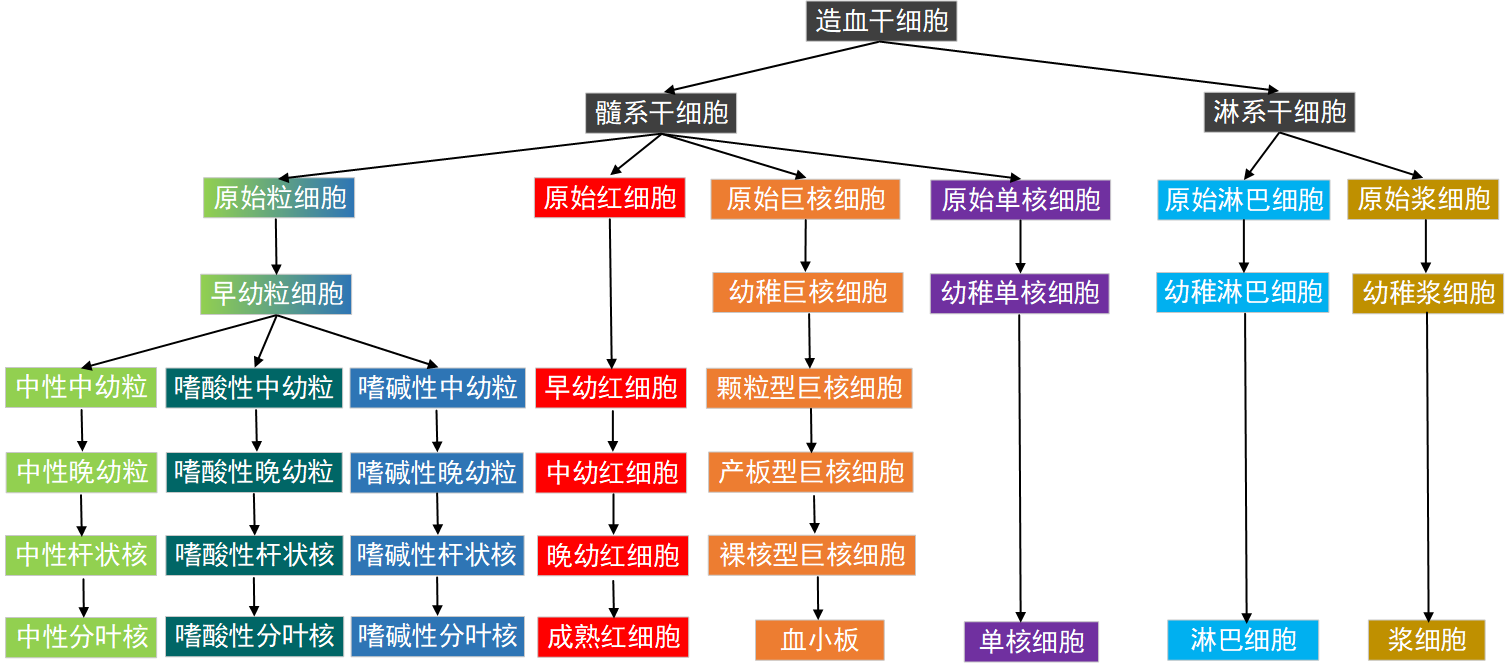
\includegraphics[width=1.0\linewidth]{development.png}
  \caption{骨髓血细胞发育成熟过程示意图}
  \label{fig:development}
\end{figure}

% \begin{itemize}
%   \item 原始细胞:胞体类圆形,直径在10\textasciitilde20微米。细胞核居中,呈圆形,染色质为粗细颗粒状,具有多个小而清晰的核仁。细胞质较少,无颗粒,呈蓝色或深蓝色。
%   \item 单核细胞:胞体呈现圆形或椭圆形,直径在14\textasciitilde25微米。细胞核扭曲折叠,常位于胞体中央或一侧,染色质疏松,核仁消失。细胞质通常为浅灰蓝色,可见空泡与紫红色的粉尘样颗粒。
%   \item 淋巴细胞:胞体为类圆形或不规则,直径在12\textasciitilde15微米。细胞核染色质致密,呈现索块状,形态上存在凹陷或者切迹。细胞质极少,呈现淡蓝色无颗粒。
%   \item 浆细胞:胞体常呈椭圆形或不规则,直径在12\textasciitilde16微米。细胞核多偏位,染色质聚集。细胞质为不透明的深蓝色,在细胞核周有淡染色带。
%   \item 有核红细胞:胞体规则类圆形,直径在7\textasciitilde10微米。细胞核为圆形位于细胞中央,内部含多个紫黑色团块。细胞质较多,无颗粒,为淡红色。
%   \item 早幼粒细胞:胞体较大,圆形或椭圆形,直径在12\textasciitilde25微米。细胞核较大,内部染色质细致,有清晰可见的核仁。细胞质为深蓝色,含有分布不均、形态不一的非特异性颗粒。
%   \item 中性中幼粒细胞:胞体为类圆形,直径在10\textasciitilde20微米。细胞核为半圆形或微凹陷,无核仁,染色质密集索块状。细胞质呈淡蓝色,其中存在大小均一,密集的淡粉红色中性颗粒。
%   \item 中性晚幼粒细胞:胞体类圆形,直径在10\textasciitilde16微米。细胞核呈半月形,存在凹陷,凹陷程度小于直径的1/2。染色质聚集小块状。细胞质多,淡蓝色,存在较多中性颗粒。
%   \item 中性杆状核细胞:胞体类圆形,直径10\textasciitilde15微米。细胞核为杆状、S形、U形等,凹陷程度大于直径的1/2,染色质粗块状。细胞质丰富,淡蓝色,充满中性颗粒。
%   \item 中性分页核细胞:胞体类圆形,直径10\textasciitilde14微米。细胞核通常分为2-5叶,之间通过核丝连接。细胞质丰富含有较多中性颗粒。
%   \item 嗜酸性粒细胞:胞体直径15\textasciitilde20微米。特点类似中性粒细胞,细胞质中存在大小分布均一,橘红色的嗜酸性颗粒。
% \end{itemize}
不同类别的骨髓血细胞胞体形状各异且细胞核与细胞浆会呈现出不同的颜色与纹理特征。表~\ref{table:cell_feature}
对本文主要关注的骨髓血细胞类别进行细胞核、细胞质等形态学方面的简要介绍。
\begin{longtable}{ccccc}
  % \centering
  \caption[Short Caption]{骨髓血细胞形态学特征}
  \label{table:cell_feature} \\
  % 下面是表头
  \hline
  \textbf{细胞名称} & \textbf{图像示例} & \textbf{胞体特征} & \textbf{细胞核} & \textbf{细胞质} \\ 
  \hline 
  \endfirsthead
  % 下面数字3的意思是表格的列数
  \multicolumn{5}{c}%
  {{\tablename\ \thetable{} --接上表}} \\
  \hline 
  \textbf{细胞名称} & \textbf{图像示例} & \textbf{胞体特征} & \textbf{细胞核} & \textbf{细胞质} \\ 
  \hline  
  % 注意这里把表头复制了一遍,因为在新的页面也会展示一下表头,不然表格不方便阅读
  \endhead
  \hline 
  % \multicolumn{5}{r}{{骨髓血细胞形态学特征}} \\ \hline
  \endfoot
  \endlastfoot
  原始细胞 & 
  \multicolumn{1}{m{0.15\textwidth}}{
  \begin{minipage}[b]{0.15\textwidth}
      \centering
      {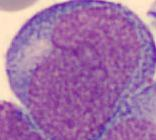
\includegraphics[width=0.9\textwidth]{cell_example/原始细胞.jpg}}
  \end{minipage}} &  
  \multicolumn{1}{m{0.15\textwidth}}{类圆形,直径10\textasciitilde20微米} & 
  \multicolumn{1}{m{0.20\textwidth}}{居中,呈圆形,染色质为颗粒状,具有多个小而清晰的核仁} & 
  \multicolumn{1}{m{0.20\textwidth}}{细胞质较少,无颗粒,呈蓝色或深蓝色}\\
  \midrule[0.5pt]
  单核细胞 & 
  \multicolumn{1}{m{0.15\textwidth}}{
  \begin{minipage}[b]{0.15\textwidth}
      \centering
      {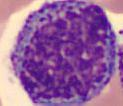
\includegraphics[width=0.9\textwidth]{cell_example/单核细胞.jpg}}
  \end{minipage}} &  
  \multicolumn{1}{m{0.15\textwidth}}{圆形或椭圆形,直径在14\textasciitilde25微米} & 
  \multicolumn{1}{m{0.20\textwidth}}{扭曲折叠,常位于胞体中央或一侧,染色质疏松,核仁消失} & 
  \multicolumn{1}{m{0.20\textwidth}}{通常为浅灰蓝色,可见空泡与紫红色的粉尘样颗粒}\\
  \midrule[0.5pt]
  淋巴细胞 & 
  \multicolumn{1}{m{0.15\textwidth}}{
  \begin{minipage}[b]{0.15\textwidth}
      \centering
      {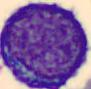
\includegraphics[width=0.9\textwidth]{cell_example/淋巴细胞.jpg}}
  \end{minipage}} &  
  \multicolumn{1}{m{0.15\textwidth}}{类圆形或不规则,直径在12\textasciitilde15微米} & 
  \multicolumn{1}{m{0.20\textwidth}}{染色质致密,呈现索块状,形态上存在凹陷或者切迹} & 
  \multicolumn{1}{m{0.20\textwidth}}{细胞质极少,呈现淡蓝色,无颗粒。}\\
  \midrule[0.5pt]
  浆细胞 & 
  \multicolumn{1}{m{0.15\textwidth}}{
  \begin{minipage}[b]{0.15\textwidth}
      \centering
      {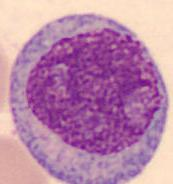
\includegraphics[width=0.9\textwidth]{cell_example/浆细胞.jpg}}
  \end{minipage}} &  
  \multicolumn{1}{m{0.15\textwidth}}{椭圆形或不规则,直径在12\textasciitilde16微米} & 
  \multicolumn{1}{m{0.20\textwidth}}{多偏位,染色质聚集} & 
  \multicolumn{1}{m{0.20\textwidth}}{细胞质为不透明的深蓝色,在细胞核周有淡染色带}\\
  \midrule[0.5pt]
  有核红细胞 & 
  \multicolumn{1}{m{0.15\textwidth}}{
  \begin{minipage}[b]{0.15\textwidth}
      \centering
      {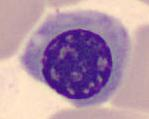
\includegraphics[width=0.9\textwidth]{cell_example/红细胞.jpg}}
  \end{minipage}} &  
  \multicolumn{1}{m{0.15\textwidth}}{规则类圆形,直径在7\textasciitilde10微米} & 
  \multicolumn{1}{m{0.20\textwidth}}{圆形位于细胞中央,内部含多个紫黑色团块} & 
  \multicolumn{1}{m{0.20\textwidth}}{细胞质较多,无颗粒,为淡红色。}\\
  \midrule[0.5pt]
  早幼粒细胞 & 
  \multicolumn{1}{m{0.15\textwidth}}{
  \begin{minipage}[b]{0.15\textwidth}
      \centering
      {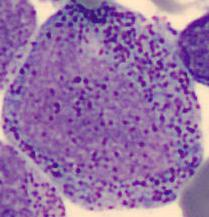
\includegraphics[width=0.9\textwidth]{cell_example/早幼粒细胞.jpg}}
  \end{minipage}} &  
  \multicolumn{1}{m{0.15\textwidth}}{较大,圆形或椭圆形,直径在12\textasciitilde25微米} & 
  \multicolumn{1}{m{0.20\textwidth}}{核较大,内部染色质细致,有清晰可见的核仁} & 
  \multicolumn{1}{m{0.20\textwidth}}{细胞质为深蓝色,含有分布不均、形态不一的非特异性颗粒}\\
  \midrule[0.5pt]
  中性中幼粒细胞 & 
  \multicolumn{1}{m{0.15\textwidth}}{
  \begin{minipage}[b]{0.15\textwidth}
      \centering
      {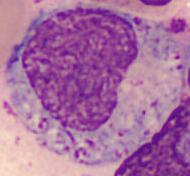
\includegraphics[width=0.9\textwidth]{cell_example/中幼粒细胞.jpg}}
  \end{minipage}} &  
  \multicolumn{1}{m{0.15\textwidth}}{类圆形,直径在10\textasciitilde20微米} & 
  \multicolumn{1}{m{0.20\textwidth}}{半圆形或微凹陷,无核仁,染色质密集索块状} & 
  \multicolumn{1}{m{0.20\textwidth}}{细胞质呈淡蓝色,其中存在大小均一,密集的淡粉红色中性颗粒}\\
  \midrule[0.5pt]
  中性晚幼粒细胞 & 
  \multicolumn{1}{m{0.15\textwidth}}{
  \begin{minipage}[b]{0.15\textwidth}
      \centering
      {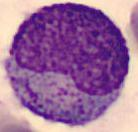
\includegraphics[width=0.9\textwidth]{cell_example/中性晚幼粒.jpg}}
  \end{minipage}} &  
  \multicolumn{1}{m{0.15\textwidth}}{胞体类圆形,直径在10\textasciitilde16微米} & 
  \multicolumn{1}{m{0.20\textwidth}}{呈半月形,存在凹陷,凹陷程度小于直径的1/2,染色质聚集小块状} & 
  \multicolumn{1}{m{0.20\textwidth}}{细胞质多,淡蓝色,存在较多中性颗粒}\\
  \midrule[0.5pt]
  中性晚幼粒细胞 & 
  \multicolumn{1}{m{0.15\textwidth}}{
  \begin{minipage}[b]{0.15\textwidth}
      \centering
      {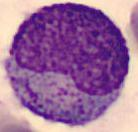
\includegraphics[width=0.9\textwidth]{cell_example/中性晚幼粒.jpg}}
  \end{minipage}} &  
  \multicolumn{1}{m{0.15\textwidth}}{胞体类圆形,直径在10\textasciitilde16微米} & 
  \multicolumn{1}{m{0.20\textwidth}}{呈半月形,存在凹陷,凹陷程度小于直径的1/2,染色质聚集小块状} & 
  \multicolumn{1}{m{0.20\textwidth}}{细胞质多,淡蓝色,存在较多中性颗粒}\\
  \midrule[0.5pt]
  中性杆状核细胞 & 
  \multicolumn{1}{m{0.15\textwidth}}{
  \begin{minipage}[b]{0.15\textwidth}
      \centering
      {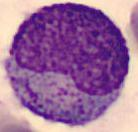
\includegraphics[width=0.9\textwidth]{cell_example/中性晚幼粒.jpg}}
  \end{minipage}} &  
  \multicolumn{1}{m{0.15\textwidth}}{胞体类圆形,直径在10\textasciitilde16微米} & 
  \multicolumn{1}{m{0.20\textwidth}}{呈半月形,存在凹陷,凹陷程度小于直径的1/2,染色质聚集小块状} & 
  \multicolumn{1}{m{0.20\textwidth}}{细胞质多,淡蓝色,存在较多中性颗粒}\\
  \midrule[0.5pt]
  中性分页核细胞 & 
  \multicolumn{1}{m{0.15\textwidth}}{
  \begin{minipage}[b]{0.15\textwidth}
      \centering
      {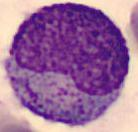
\includegraphics[width=0.9\textwidth]{cell_example/中性晚幼粒.jpg}}
  \end{minipage}} &  
  \multicolumn{1}{m{0.15\textwidth}}{胞体类圆形,直径在10\textasciitilde16微米} & 
  \multicolumn{1}{m{0.20\textwidth}}{呈半月形,存在凹陷,凹陷程度小于直径的1/2,染色质聚集小块状} & 
  \multicolumn{1}{m{0.20\textwidth}}{细胞质多,淡蓝色,存在较多中性颗粒}\\
  \midrule[0.5pt]
  嗜酸性粒细胞 & 
  \multicolumn{1}{m{0.15\textwidth}}{
  \begin{minipage}[b]{0.15\textwidth}
      \centering
      {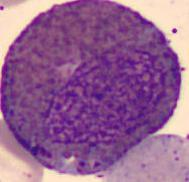
\includegraphics[width=0.9\textwidth]{cell_example/嗜酸性.jpg}}
  \end{minipage}} &  
  \multicolumn{1}{m{0.15\textwidth}}{直径15\textasciitilde20微米。} & 
  \multicolumn{1}{m{0.20\textwidth}}{类似中性粒细胞,染色质聚集索块} & 
  \multicolumn{1}{m{0.20\textwidth}}{大小分布均一,橘红色的嗜酸性颗粒}\\
  \midrule[0.5pt]
  嗜碱性粒细胞 & 
  \multicolumn{1}{m{0.15\textwidth}}{
  \begin{minipage}[b]{0.15\textwidth}
      \centering
      {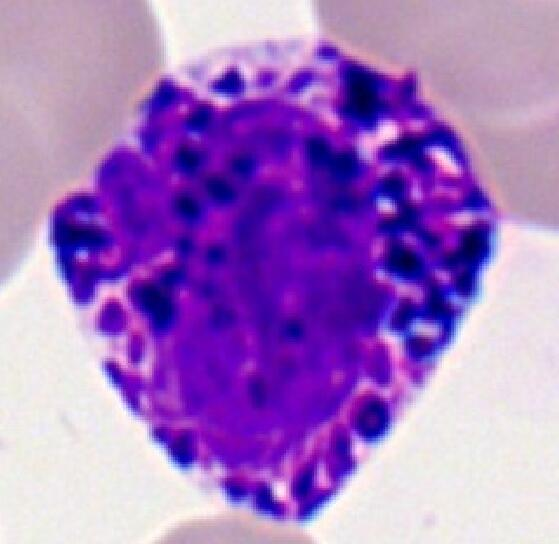
\includegraphics[width=0.9\textwidth]{cell_example/嗜碱性.jpg}}
  \end{minipage}} &  
  \multicolumn{1}{m{0.15\textwidth}}{直径10\textasciitilde15微米。} & 
  \multicolumn{1}{m{0.20\textwidth}}{染色质细致} & 
  \multicolumn{1}{m{0.20\textwidth}}{颗粒粗大,大小形态不一深紫红色的颗粒,部分颗粒覆盖在细胞核上}\\
  \bottomrule[1.5pt]
  \end{longtable}
\subsection{骨髓血细胞数据集与预处理}

\textbf{1)骨髓血细胞切片与数字化}

骨髓血细胞形态学检验技术是临床诊断血液疾病的重要依据。该过程由取材、制片、固定、染色、洗涤干燥与镜检等流程组成。首先通过骨髓穿刺采集骨髓液样本。接着将骨髓液
置于载玻片上制作成薄厚均一的涂片。在涂片制作完成后,使用甲醛或乙醇溶液将其固定。然后采用瑞特-吉姆萨染色剂进行适当时间的着色,染色完成后使用清水冲洗,待自然风干后以备观察。
最后使用光学显微镜对骨髓涂片进行观察,统计骨髓中不同类型血细胞的数量、比例,形态以及是否存在异常细胞,进行骨髓评估判断病情。具体如图~\ref{fig:cell_pre}所示:

\begin{figure}[htbp]
	\centering
	\begin{subfigure}{0.325\linewidth}
		\centering
		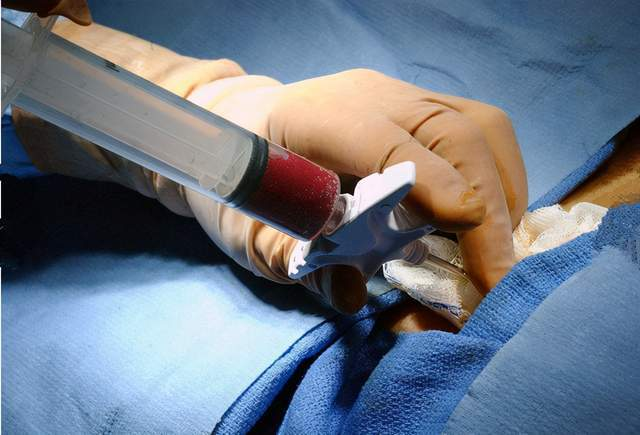
\includegraphics[width=0.95\linewidth, height=0.7\linewidth]{cell_pre/step1.jpg}
    \caption{}
	\end{subfigure}
	\centering
	\begin{subfigure}{0.325\linewidth}
		\centering
		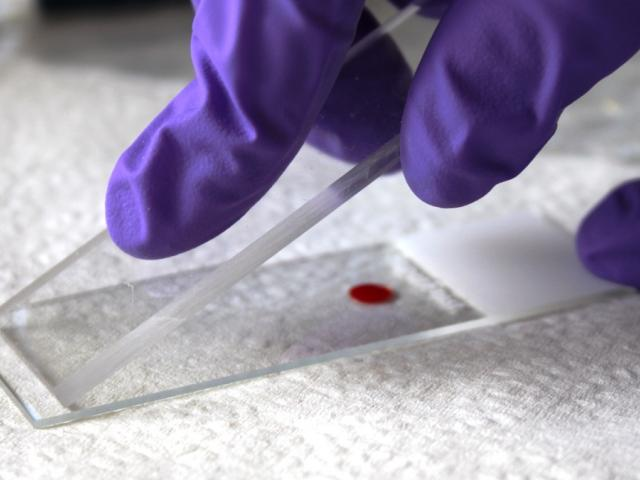
\includegraphics[width=0.95\linewidth, height=0.7\linewidth]{cell_pre/step2.jpg}
    \caption{}
	\end{subfigure}
	\centering
	\begin{subfigure}{0.325\linewidth}
		\centering
		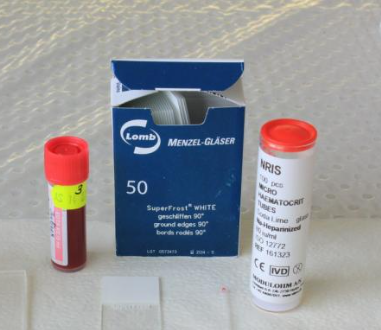
\includegraphics[width=0.95\linewidth, height=0.7\linewidth]{cell_pre/step3.jpg}
    \caption{}
	\end{subfigure}

	\centering
	\begin{subfigure}{0.325\linewidth}
		\centering
		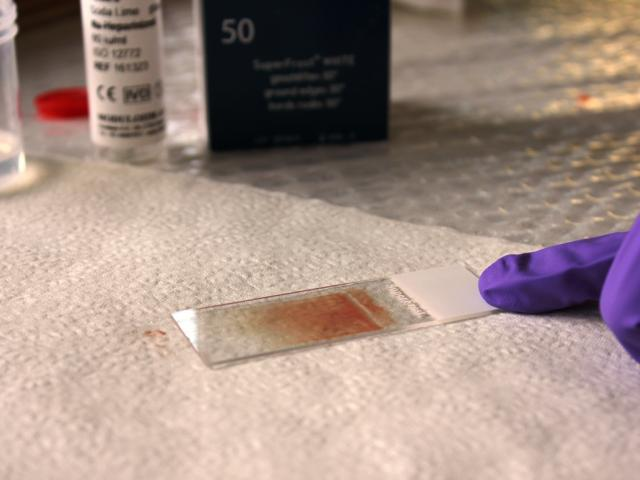
\includegraphics[width=0.95\linewidth, height=0.7\linewidth]{cell_pre/step4.jpg}
    \caption{}
	\end{subfigure}
	\centering
	\begin{subfigure}{0.325\linewidth}
		\centering
		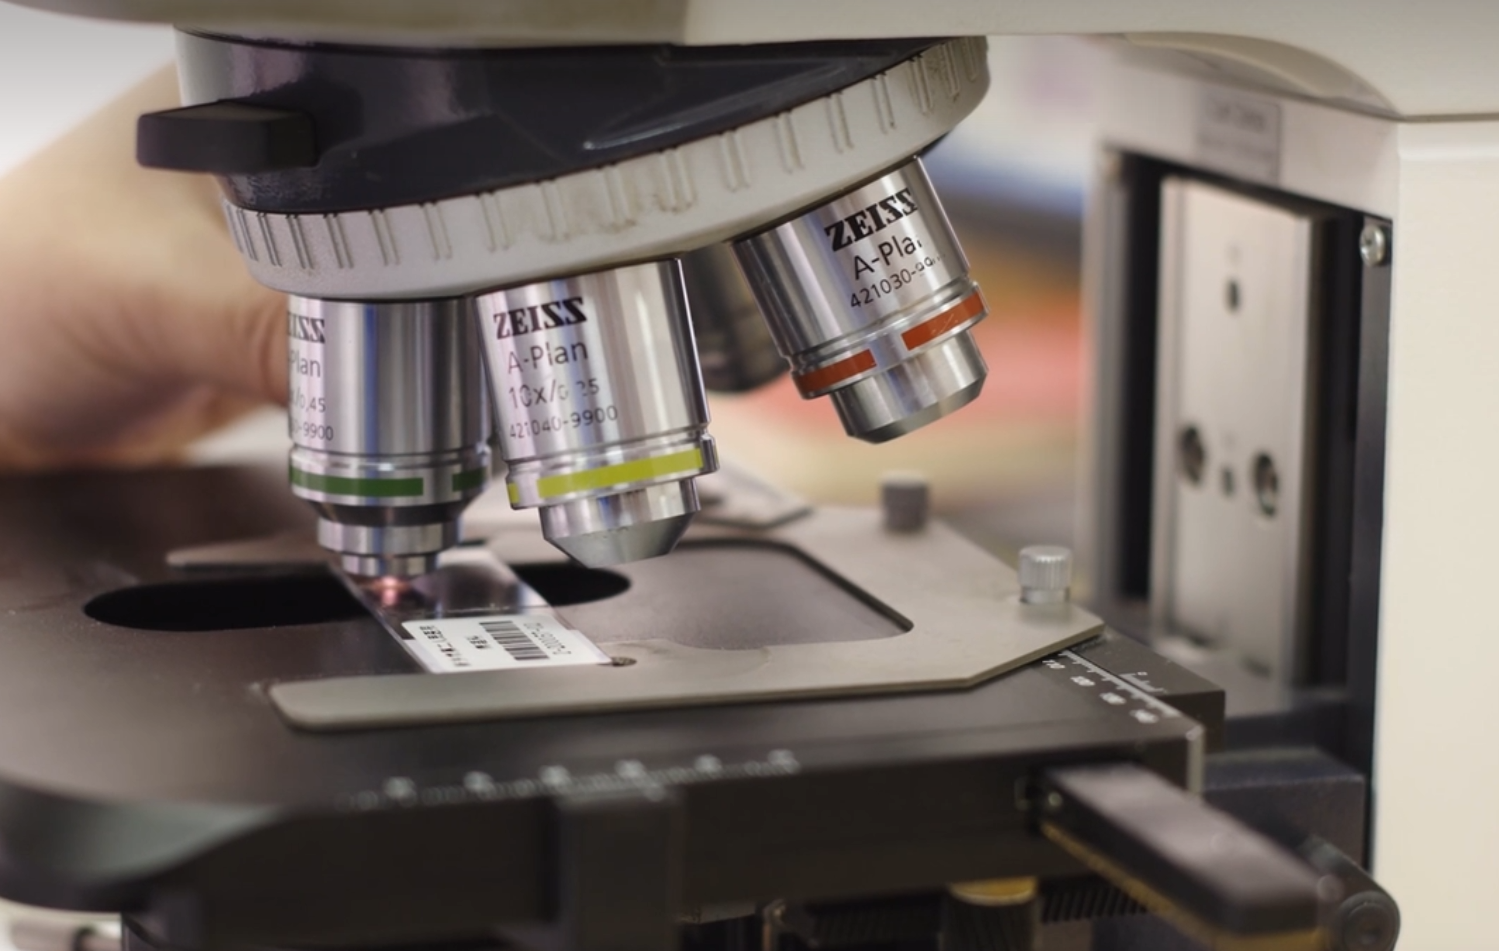
\includegraphics[width=0.95\linewidth, height=0.7\linewidth]{cell_pre/step5.jpg}
    \caption{}
	\end{subfigure}
	\centering
	\begin{subfigure}{0.325\linewidth}
		\centering
		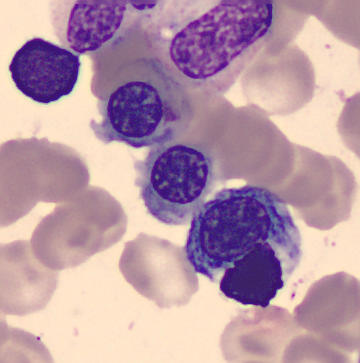
\includegraphics[width=0.95\linewidth, height=0.7\linewidth]{cell_pre/step6.jpg}
    \caption{}
	\end{subfigure}
	\caption{骨髓血细胞检验技术流程:(a)骨髓穿刺抽取骨髓液,(b)制备骨髓涂片,(c)瑞特-吉姆萨染色,(d)清洗晾干,(e)人工镜检判读,(f)骨髓形态学图片}
	\label{fig:cell_pre}
\end{figure}

对骨髓血细胞切片图像进行自动化评估分析首先需要对切片图像进行数字化,从而可以在计算机上进行存储,传输与分析。数字化技术可以为医学研究提供大量数据源,
促进医学研究与临床实验,方便医生进行更加快速与精准的病情分析。病理图像数字化技术由以下几个步骤组成。1)数字扫描:对制备好的组织切片使用数字成像与扫描设备生成数字图像,
一般通过CCD相机采用对焦深度法自动获取对焦位置并扫描成像。2)数字化处理:对图像进行去噪、分割与边缘检测等进一步提升图像质量。3)云存储与管理,将数字化图像存储在
云端服务器中,保证数据的完整性与安全。4)数字分析与诊断,利用计算机视觉等深度学习图像分析技术,对数字化后的病理图像进行分析与诊断,提高病理诊断的效率与准确性。

\textbf{2)数据集标注}

本文使用数据来源于实践基地邃蓝智能科技有限公司合作医院提供的脱敏数据。
数据标注是深度学习模型训练的基础,并且直接影响模型的性能和泛化能力。我们在合作医院病理医师的协作下对血细胞的边界框与类别信息进行精准的标注,完成了骨髓血细胞数据集(BMCD, Bone Marrow Cell Dataset)的制作。
原始数据集总共包含9250张骨髓血细胞图像,我们只关注图像中的有核细胞,而将成熟红细胞作为背景。因为缺少相关专业知识,我们仅标记出血细胞边界框的位置。
我们使用labelme软件作为标注工具,如图~\ref{fig:annotations}所示,针对每一张图像生成json标注文件,记录血细胞边界框的左上角与右下角的坐标,最后再将标注转化为coco格式,并将数据集划分为训练集、测试集与验证集。
经过检测网络,我们得到了单一血细胞图像,即图像中仅有一个完整的骨髓血细胞,这些图像再由经验丰富的病理医生完成类别标签的标注。


\begin{figure}
  \centering
  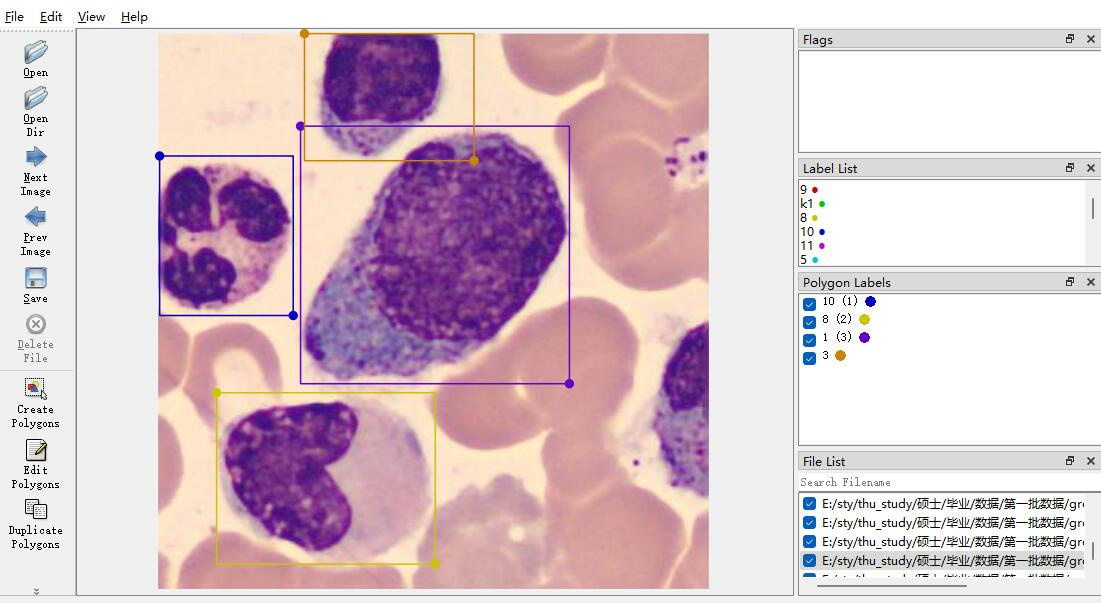
\includegraphics[width=0.8\linewidth]{annotations.jpg}
  \caption{labelme标注软件工具}
  \label{fig:annotations}
\end{figure}

大量的数据标注需要消耗很高的人力物力成本,我们采用主动学习技术去发掘数据集中高信息量的样本,提高标注的效率与精度,降低标注成本。
主动学习的基本思想是标注少量部分数据,利用已标注的数据训练深度学习模型。然后使用模型对未标注的数据进行预测,根据最大化熵、不确定度采样等进行排序,
筛选出不确定性最高的一些数据优先进行标注。不断迭代上述过程,直到标注与模型性能达到预期。具体而言,对于血细胞检测任务,首先标注将部分图像,然后训练Faster-RCNN网络
得到一个初步的检测模型,然后对每张图像进行检测,并生成标注json文件,再反馈到labelme标注软件中进行微调。针对血细胞识别任务,经过检测网络,我们得到了多张单个血细胞图像,首先完成部分
类别标注,训练初步的识别网络。对未标注的血细胞筛选出熵最大的预测样本反馈给病理医生进行核对。主动学习流程如图~\ref{fig:active}所示:

\begin{figure}
  \centering
  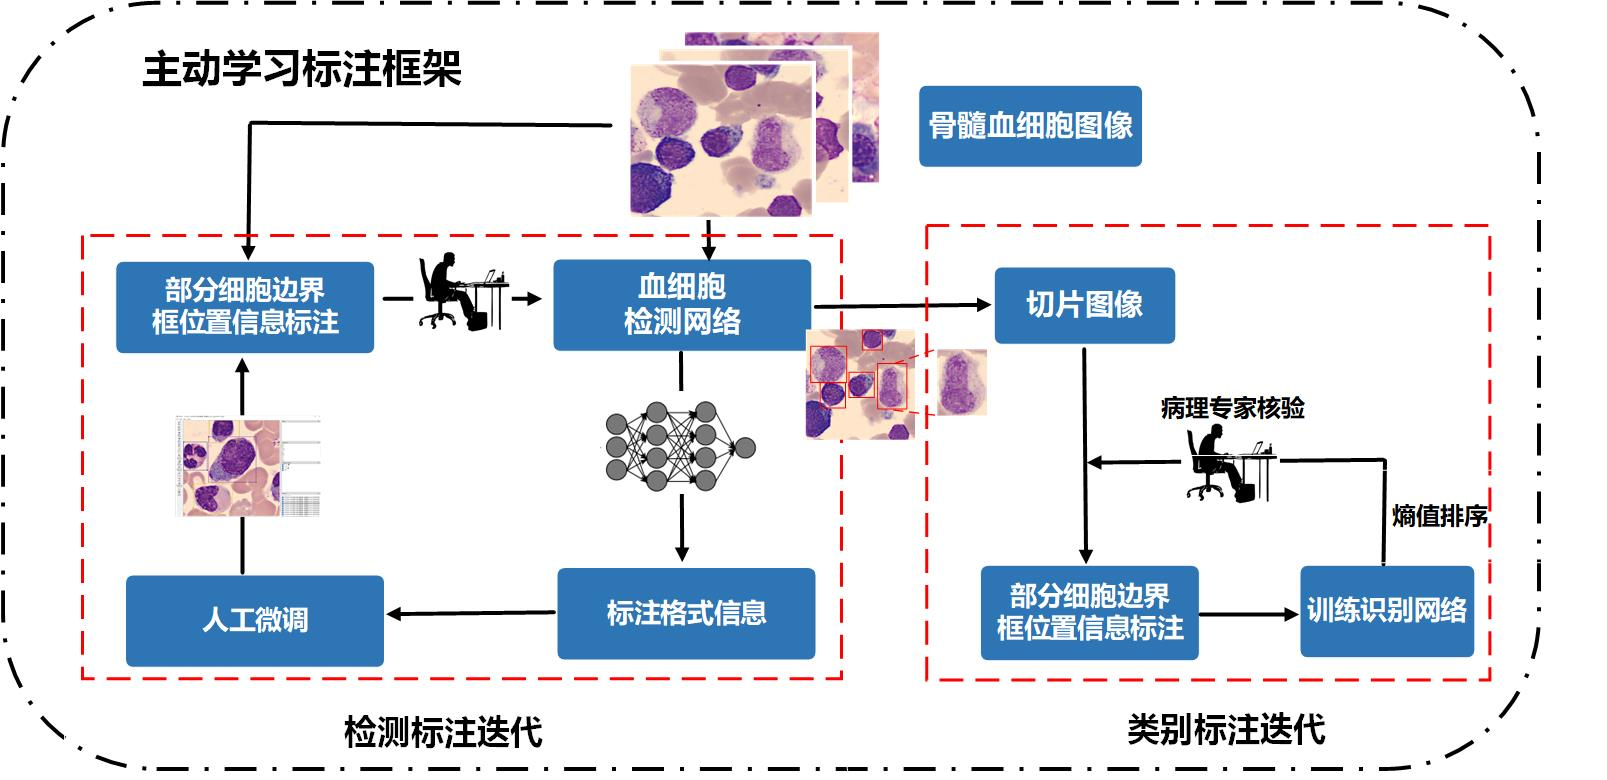
\includegraphics[width=1.0\linewidth]{active.jpg}
  \caption{主动学习标注框架示意图}
  \label{fig:active}
\end{figure}
\textbf{3)数据增强}

我们主要关注的五大系统细胞在人体内占比不同,粒细胞系统约占全部细胞的50\%,而浆细胞系统一般占比小于1.5\%,由于细胞天然就存在比例不均衡问题,其也导致了我们的数据集
存在严重的类别不平衡问题。例如单核细胞数量仅为有核红细胞数量的1/9。数据的不平衡会导致网络过多的关注数量较多的类别特征信息,数量较少类别易出现准确率与召回率的不均衡,影响模型的泛化性能。
为解决上述问题,本文对于数量较多的类别采用随机欠采样减少样本数量。对于数量较少的类别,采用翻转、旋转、添加噪声与色彩调整增加数据多样性。下面对数据增强方法进行简要介绍:
1)翻转:将图像沿水平或垂直方向进行镜像对称,生成新的图像。当图像$I(x,y)$沿水平方向进行翻转后,水平翻转图像为$I’(x, y)=I(w-x-1,y)$,其中w为原始图像宽度。
2)旋转:将图像沿着某个点或轴进行旋转,当图像$I(x,y)$以$(c_x, c_y)$为旋转中心时,旋转角度为$\theta$, 旋转后的图像为$I’(x, y)=I((x - c_x)\cos\theta - (y - c_y)\sin\theta + c_x, (x - c_x)\sin\theta - (y - c_y)\cos\theta + c_y)$。
3)添加噪声:常用的图像噪声包括高斯噪声、椒盐噪声与泊松噪声。高斯噪声是一种连续随机噪声,服从零均值、标准差为$\sigma$的正态分布,会使得图像变模糊。
椒盐噪声是离散随机噪声,图像中会出现亮点与暗点,降低图像的清晰度与对比。
4)色彩调整:常用方法包括了亮度调整、对比度调整、色相调整与饱和度调整。

\section{神经网络技术概述}
\subsection{神经元与梯度优化}

\textbf{1)神经元}

神经网络发展历史最早可以追溯到20世纪五十年代,当时研究人员受到神经科学启发,模拟生物神经元结构提出了神经网络。
神经元是神经网络的基本单元,其结构如图~\ref{fig:neuron}所示,由输入、加权、激活函数、输出这四个部分组成。
\begin{figure}
  \centering
  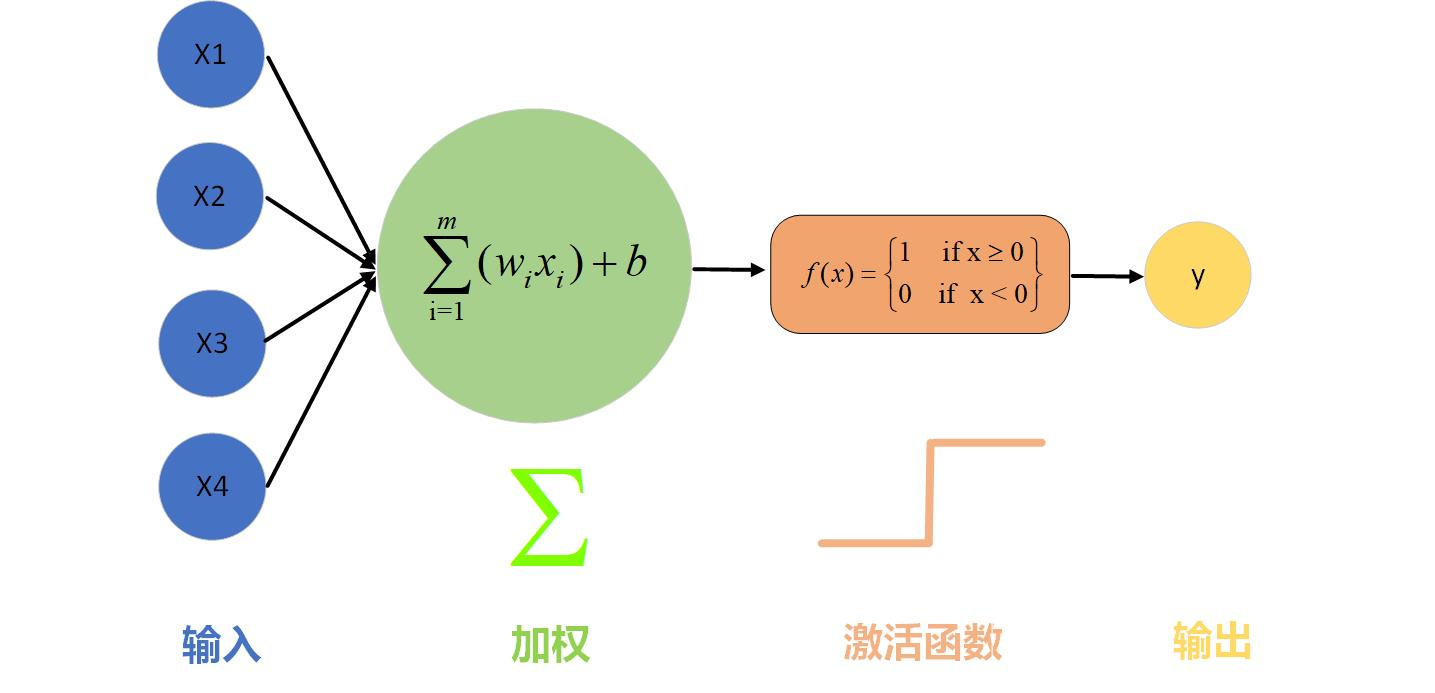
\includegraphics[width=0.8\linewidth]{neuron.jpg}
  \caption{神经元结构示意图}
  \label{fig:neuron}
\end{figure}

输入部分,神经元接收其他神经元的信息$x_1, x_2, \dots, x_4$,每个输入与权重进行关联。加权部分表示神经元对于输入部分的敏感程度。
激活函数将加权和进行变换,保证输出数值范围并引入非线性的特性。输出部分是激活函数处理后的结果,如式~\ref{eq:neuron}所示,可作为后续神经元的输入。

\begin{equation}
  h(x) = f({{\bf{W}}^T}{\bf{x}}) = f(\sum\limits_{i = 1}^m {{w_i}{x_i} + b})
  \label{eq:neuron}
\end{equation}

式~\ref{eq:neuron}中$f(\cdot)$为激活函数。常用的激活函数有修正线性单元函数(Rectified linear unit function,ReLU)、双曲正切函数、sigmoid函数等。

\textbf{2)感知机}

感知机由美国心理学家弗兰克·罗森布\cite{1958perceptron}在1958年提出,它是一种最简单的神经网络,拓扑结构如图~\ref{fig:perceptron}所示。
网络包含了输入层、隐含层与输出层,前一层的每个神经元都与后一层的神经元相连。前一层神经元输出信息传递到下一层神经元的过程称为前向传播。
该过程可以用一系列矩阵乘法与激活函数进行描述,若输入数据为$x$, 网络结构总共有$L$层,则前向传播过程可以表示为:

\begin{equation}
  \begin{aligned}
  z^{1} & =W^{1} x+b^{1} \\
  a^{1} & =g^{1}\left(z^{1}\right) \\
  & \vdots \\
  z^{L} & =W^{L} a^{L-1}+b^{L} \\
  a^{L} & =g^{L}\left(z^{L}\right)=\hat{y}
  \label{eq:perceptron}
\end{aligned}
\end{equation}

其中 $z^{l}$ 表示第$l$层的未激活值,$a^{l}$ 表示第$l$层的激活值,$W^{l}$ 和 $b^{l}$ 分别表示第$l$层的权重矩阵和偏置向量。
\begin{figure}
  \centering
  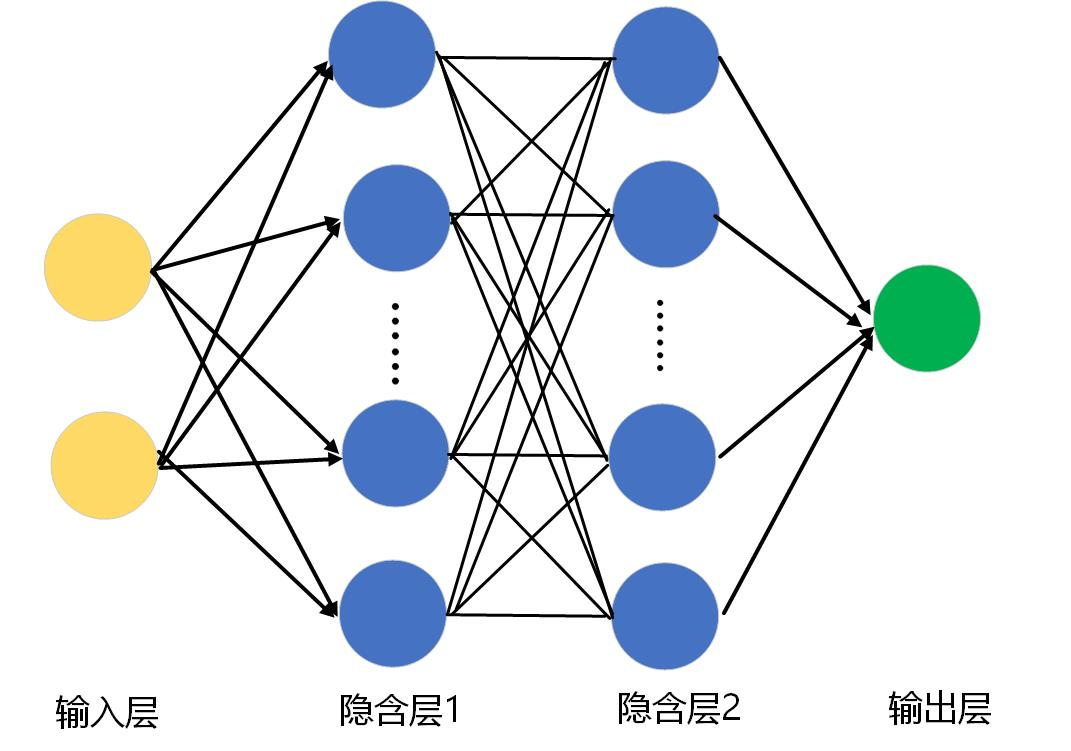
\includegraphics[width=0.65\linewidth]{perceptron.jpg}
  \caption{感知机网络模型示意图}
  \label{fig:perceptron}
\end{figure}

\textbf{3)反向传播与梯度优化}

反向传播全称是误差反向传播(back propgation,BP),是用于神经网络训练的算法。神经网络经过前向传播得到网络预测值,采用
损失函数衡量预测值与真实值之间的误差。通过损失函数最小化计算神经网络参数的导数,然后调整更新神经网络权重参数以减小误差。不断迭代上述过程,
直到模型参数收敛。

假设 $L$ 为损失函数,$w_{ij}^k$ 表示第$k$层第$i$个神经元到第$j$个神经元之间的权重,$a_j^l$ 表示$l$ 层的第$j$个神经元的非激活值
$z_j$ 表示第 $j$ 层神经元输出,$\sigma_l(\cdot)$为第l层激活函数。反向传播过程计算过程如下:
\begin{enumerate}[label=(\alph*)]
  \item 网络进行前向传播得到预测值
  \item 定义输出层的误差$\delta_k^L$为损失函数对输出层非激活值的导数,如式~\ref{eq:delta}所示,
  \begin{equation}
    \delta_k^L = \frac{\partial L}{\partial a_k^L} = \frac{\partial L}{\partial z_k^L} \frac{\partial z_k^L}{\partial a_k^L}
    \label{eq:delta}
  \end{equation}
  \item 对于中间隐含层,可以通过链式法则求出第$l$层的传播误差$\delta_j^l$
  \begin{equation}
    \begin{aligned}
    \delta_j^l & = \frac{\partial L}{\partial a_j^l} = \frac{\partial L}{\partial z_j^l} \frac{\partial z_j^l}{\partial a_j^l} \\
    \frac{{\partial L}}{{\partial z_j^l}} & = \sum\limits_i^{} {\frac{{\partial L}}{{\partial a_i^{l + 1}}}} \frac{{\partial a_i^{l + 1}}}{{\partial z_j^l}} = \sum\limits_i^{} {\delta _i^{l + 1}} w_{ij}^{l + 1} \\
    \delta_j^l & = \frac{{\partial L}}{{\partial a_j^l}} = \sigma _l^\prime \left( {a_j^l} \right)\sum\limits_i^{} {w_{ij}^{l + 1}} \delta _i^{l + 1}
    \end{aligned}
    \label{eq:delta_l}
  \end{equation}
  \item 计算损失函数对于某一隐含层$l$权重$w_{ij}^k$的梯度值
  \begin{equation}
    \frac{{\partial L}}{{\partial w_{ij}^l}} = \frac{{\partial L}}{{\partial a_j^l}}\frac{{\partial a_j^l}}{{\partial w_{ij}^l}} = \delta_j^l z_i^{l - 1}
    \label{eq:delta_w}
  \end{equation}
  \item 若训练的学习率为$\eta$,随机抽取小批量样本$\left\{ {\left( {{{\bf{x}}_m},{{\bf{y}}_m}} \right)} \right\}_{m = 1}^{{N_0}}$,权重值的更新如下
  \begin{equation}
    w_{ij}^{l(\tau  + 1)} = w_{ij}^{l(\tau )} - \eta \frac{1}{{{N_0}}}\sum\limits_{m = 1}^{{N_0}} {\frac{{\partial {L_m}}}{{\partial w_{ij}^l}}}
    \label{eq:update}
  \end{equation}
  \item 重复上述步骤,直到损失函数达到极小值,得到收敛后最优的网络模型参数
\end{enumerate}




\subsection{卷积神经网络}
\subsection{训练方法}

\section{软件设计相关技术}
\subsection{前端技术}
\subsection{后端技术}
\subsection{Mysql数据库}

% 图片通常在 \env{figure} 环境中使用 \cs{includegraphics} 插入,如图~\ref{fig:example} 的源代码。
% 建议矢量图片使用 PDF 格式,比如数据可视化的绘图;
% 照片应使用 JPG 格式;
% 其他的栅格图应使用无损的 PNG 格式。
% 注意,LaTeX 不支持 TIFF 格式;EPS 格式已经过时。

% \begin{figure}
%   \centering
%   
\includegraphics[width=0.5\linewidth]{example-image-a.pdf}
%   \caption*{国外的期刊习惯将图表的标题和说明文字写成一段,需要改写为标题只含图表的名称,其他说明文字以注释方式写在图表下方,或者写在正文中。}
%   \caption{示例图片标题}
%   \label{fig:example}
% \end{figure}

% 若图或表中有附注,采用英文小写字母顺序编号,附注写在图或表的下方。
% 国外的期刊习惯将图表的标题和说明文字写成一段,需要改写为标题只含图表的名称,其他说明文字以注释方式写在图表下方,或者写在正文中。

% 如果一个图由两个或两个以上分图组成时,各分图分别以 (a)、(b)、(c)...... 作为图序,并须有分图题。
% 推荐使用 \pkg{subcaption} 宏包来处理, 比如图~\ref{fig:subfig-a} 和图~\ref{fig:subfig-b}。

% \begin{figure}
%   \centering
%   \subcaptionbox{分图 A\label{fig:subfig-a}}
%     {
\includegraphics[width=0.35\linewidth]{example-image-a.pdf}}
%   \subcaptionbox{分图 B\label{fig:subfig-b}}
%     {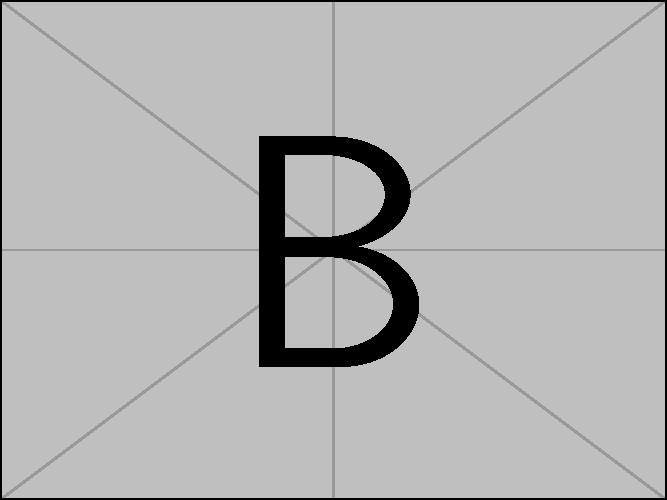
\includegraphics[width=0.35\linewidth]{example-image-b.pdf}}
%   \caption{多个分图的示例}
%   \label{fig:multi-image}
% \end{figure}



% \section{表格}

% 表应具有自明性。为使表格简洁易读,尽可能采用三线表,如表~\ref{tab:three-line}。
% 三条线可以使用 \pkg{booktabs} 宏包提供的命令生成。

% \begin{table}
%   \centering
%   \caption{三线表示例}
%   \begin{tabular}{ll}
%     \toprule
%     文件名          & 描述                         \\
%     \midrule
%     thuthesis.dtx   & 模板的源文件,包括文档和注释 \\
%     thuthesis.cls   & 模板文件                     \\
%     thuthesis-*.bst & BibTeX 参考文献表样式文件    \\
%     \bottomrule
%   \end{tabular}
%   \label{tab:three-line}
% \end{table}

% 表格如果有附注,尤其是需要在表格中进行标注时,可以使用 \pkg{threeparttable} 宏包。
% 研究生要求使用英文小写字母 a、b、c……顺序编号,本科生使用圈码 ①、②、③……编号。

% \begin{table}
%   \centering
%   \begin{threeparttable}[c]
%     \caption{带附注的表格示例}
%     \label{tab:three-part-table}
%     \begin{tabular}{ll}
%       \toprule
%       文件名                 & 描述                         \\
%       \midrule
%       thuthesis.dtx\tnote{a} & 模板的源文件,包括文档和注释 \\
%       thuthesis.cls\tnote{b} & 模板文件                     \\
%       thuthesis-*.bst        & BibTeX 参考文献表样式文件    \\
%       \bottomrule
%     \end{tabular}
%     \begin{tablenotes}
%       \item [a] 可以通过 xelatex 编译生成模板的使用说明文档;
%         使用 xetex 编译 \file{thuthesis.ins} 时则会从 \file{.dtx} 中去除掉文档和注释,得到精简的 \file{.cls} 文件。
%       \item [b] 更新模板时,一定要记得编译生成 \file{.cls} 文件,否则编译论文时载入的依然是旧版的模板。
%     \end{tablenotes}
%   \end{threeparttable}
% \end{table}

% 如某个表需要转页接排,可以使用 \pkg{longtable} 宏包,需要在随后的各页上重复表的编号。
% 编号后跟表题(可省略)和“(续)”,置于表上方。续表均应重复表头。

% \begin{longtable}{cccc}
%     \caption{跨页长表格的表题}
%     \label{tab:longtable} \\
%     \toprule
%     表头 1 & 表头 2 & 表头 3 & 表头 4 \\
%     \midrule
%   \endfirsthead
%     \caption*{续表~\thetable\quad 跨页长表格的表题} \\
%     \toprule
%     表头 1 & 表头 2 & 表头 3 & 表头 4 \\
%     \midrule
%   \endhead
%     \bottomrule
%   \endfoot
%   Row 1  & & & \\
%   Row 2  & & & \\
%   Row 3  & & & \\
%   Row 4  & & & \\
%   Row 5  & & & \\
%   Row 6  & & & \\
%   Row 7  & & & \\
%   Row 8  & & & \\
%   Row 9  & & & \\
%   Row 10 & & & \\
% \end{longtable}



% \section{算法}

% 算法环境可以使用 \pkg{algorithms} 或者 \pkg{algorithm2e} 宏包。

% \renewcommand{\algorithmicrequire}{\textbf{输入:}\unskip}
% \renewcommand{\algorithmicensure}{\textbf{输出:}\unskip}

% \begin{algorithm}
%   \caption{Calculate $y = x^n$}
%   \label{alg1}
%   \small
%   \begin{algorithmic}
%     \REQUIRE $n \geq 0$
%     \ENSURE $y = x^n$

%     \STATE $y \leftarrow 1$
%     \STATE $X \leftarrow x$
%     \STATE $N \leftarrow n$

%     \WHILE{$N \neq 0$}
%       \IF{$N$ is even}
%         \STATE $X \leftarrow X \times X$
%         \STATE $N \leftarrow N / 2$
%       \ELSE[$N$ is odd]
%         \STATE $y \leftarrow y \times X$
%         \STATE $N \leftarrow N - 1$
%       \ENDIF
%     \ENDWHILE
%   \end{algorithmic}
% \end{algorithm}
